% Copyright 2024 Fausto Spoto
%
% Licensed under the Apache License, Version 2.0 (the "License");
% you may not use this file except in compliance with the License.
% You may obtain a copy of the License at
%
%    http://www.apache.org/licenses/LICENSE-2.0
%
% Unless required by applicable law or agreed to in writing, software
% distributed under the License is distributed on an "AS IS" BASIS,
% WITHOUT WARRANTIES OR CONDITIONS OF ANY KIND, either express or implied.
% See the License for the specific language governing permissions and
% limitations under the License.

\documentclass[11pt]{beamer}  %% versione proiettore
%%\documentclass[11pt,handout]{beamer} %% versione stampa
\usepackage{lucidiJb-2ed}

\usepackage{mathtools}
\usepackage{relsize}
\usepackage[normalem]{ulem}

\mode<article>
{
  \usepackage{fullpage}
  \usepackage{hyperref}
}

\mode<presentation>
{
  \setbeamertemplate{background canvas}[vertical shading][bottom=red!10,top=blue!10]
  \usetheme{Course}
  \usefonttheme[onlysmall]{structurebold}
}

\subtitle{S\~ao Luis, Brasil, 18/6/2024}
\title{Blockchain and its Energy Cost}
\institute{Universit\`a di Verona, Italy}
\date{June 2024}

\setbeamercovered{invisible}

\def\codesize{\smaller}
\def\<#1>{\codeid{#1}}
\newcommand{\codeid}[1]{\ifmmode{\mbox{\codesize\ttfamily{#1}}}\else{\codesize\ttfamily #1}\fi}

\AtBeginSection[]{
  \begin{frame}
  \vfill
  \centering
  \begin{beamercolorbox}[sep=8pt,center,shadow=true,rounded=true]{title}
    \usebeamerfont{title}\insertsectionhead\par%
  \end{beamercolorbox}
  \vfill
  \end{frame}
}

\begin{document}

\begin{frame}
  \titlepage
\end{frame}

\begin{frame}\frametitle{Who issues and moves the money?}

  \begin{center}
    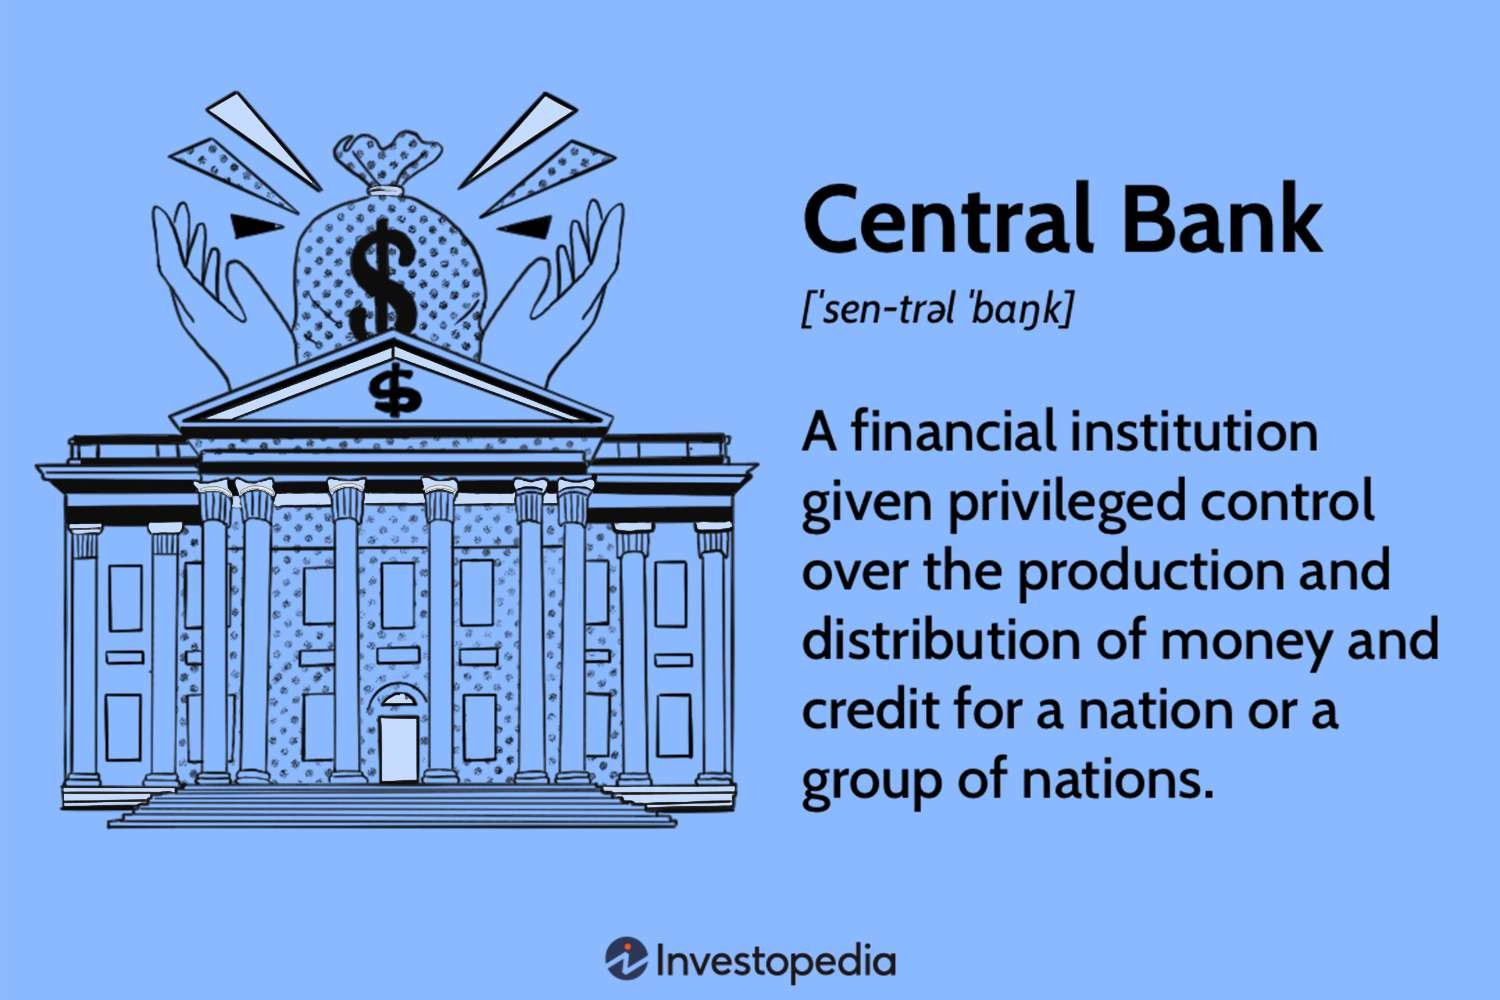
\includegraphics[scale=0.22,clip=false]{pictures/central-bank.jpg}
  \end{center}

\end{frame}

\begin{frame}\frametitle{Can I at least move the money?}

  \begin{center}
    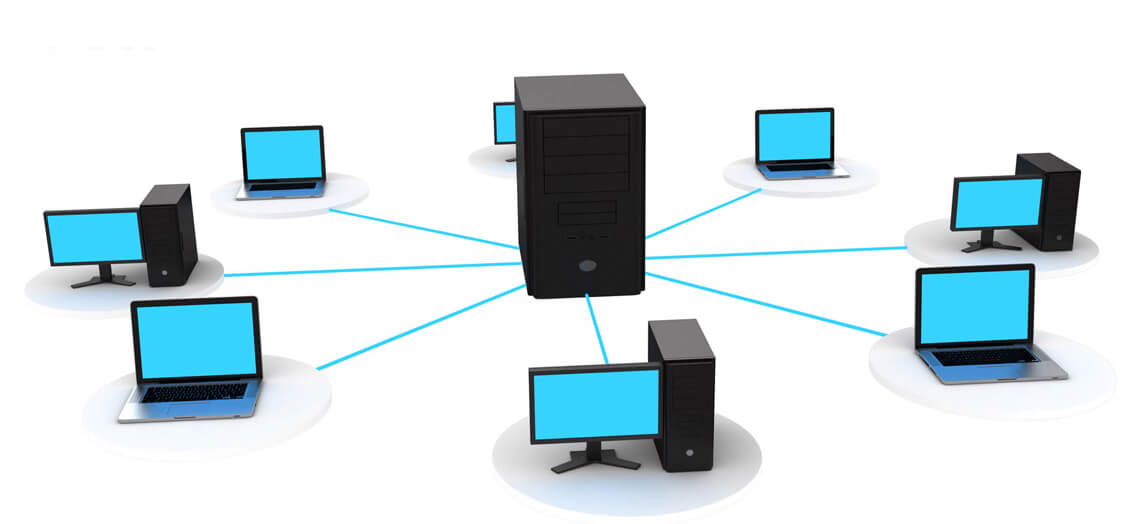
\includegraphics[scale=0.22,clip=false]{pictures/centralized-network.jpg}
  \end{center}

  \begin{greenbox}{It's all about trust}
    \begin{itemize}
    \item if my central computer crashes, data might get lost
    \item if I modify the data in my central computer, I modify
      the accounts of the users
    \end{itemize}
  \end{greenbox}
  
\end{frame}

\begin{frame}{Trust is rare in this world}

  \begin{itemize}
  \item we trust our supermarket points because they have little and limited value
  \item we trust PayPal because we keep and exchange little money on it
  \item we trust credit card issuers up to a few thousand dollars
    because they \emph{should not} fail
    and \emph{should not} cheat (too big to fail, to big to cheat)
  \end{itemize}

\end{frame}

\begin{frame}\frametitle{Can trust arise in a trusteless world?}

  \begin{greenbox}{We want a money handling system that}
    \begin{itemize}
    \item has no central, special computer
    \item consists of many computers, all created equal
    \item if some computers fail, the network survives
    \item each computer contains all data, it does not need the others
    \item if a computer holds corrupted data, we can immediately see it
    \item each single computer is very unlikely to change its data
      from a non-corrupted state to another non-corrupted state (history
      must be hard to change, no double spending)
    \end{itemize}
  \end{greenbox}

  \begin{center}
    
\includegraphics[scale=0.3,clip=false]{pictures/unicorn.jpg}
  \end{center}

\end{frame}

\begin{frame}\frametitle{Distributed network}

  \begin{center}
    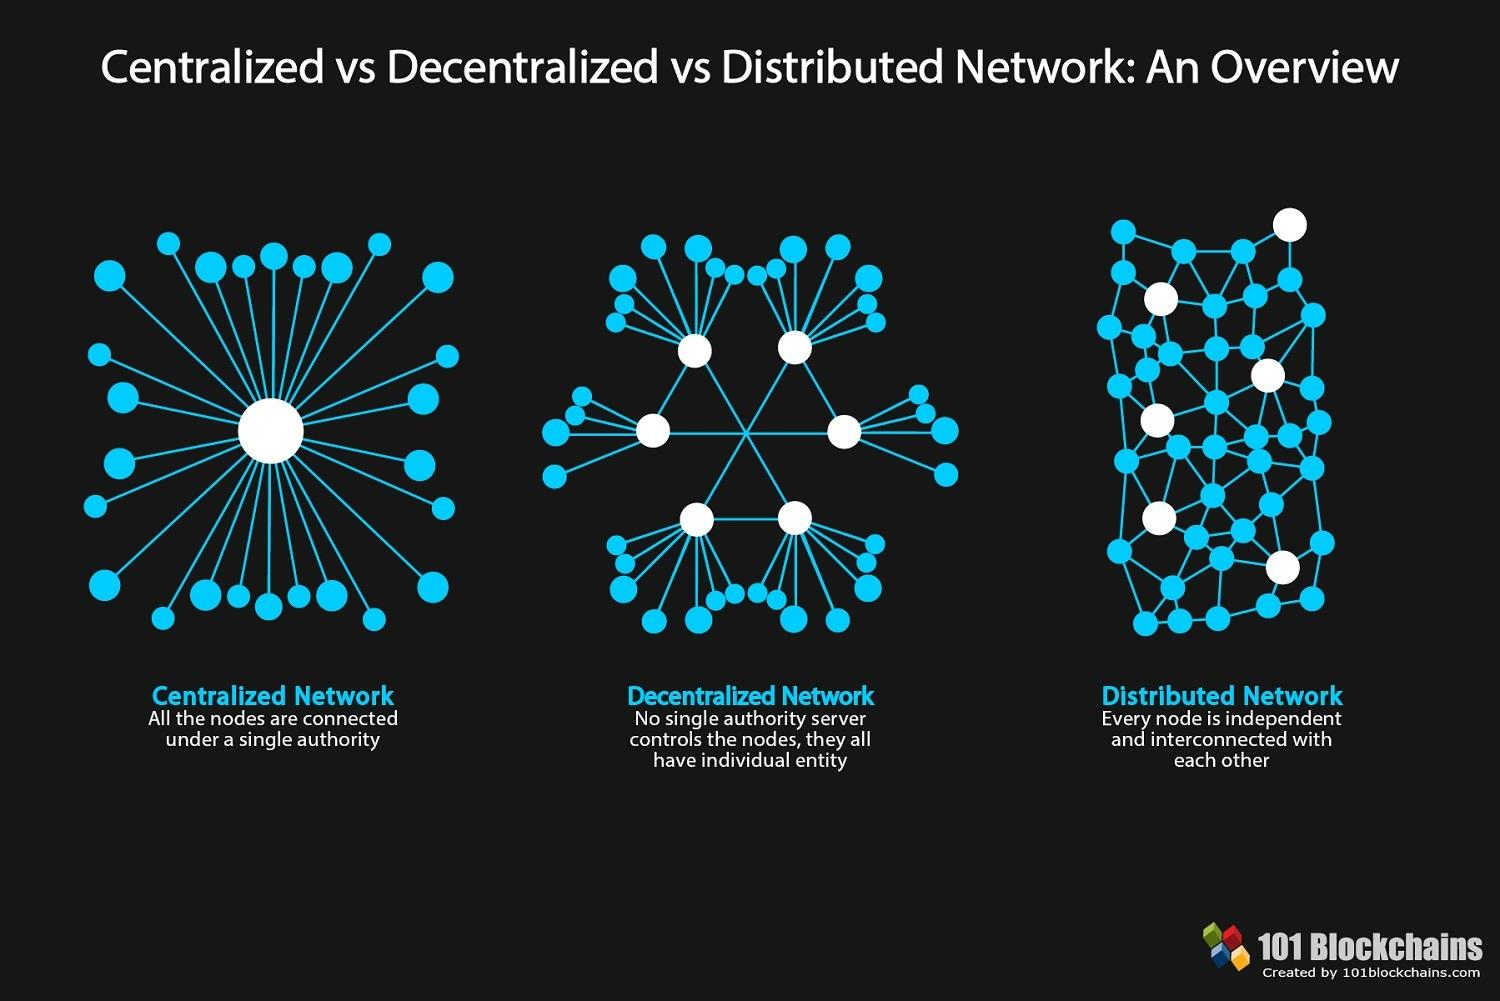
\includegraphics[scale=0.22,clip=false]{pictures/distributed.jpg}
  \end{center}

\end{frame}

\begin{frame}\frametitle{A Bit of History}

  \begin{itemize}
  \item[1991] a cryptographically secure chain of blocks (Haber \& Stornetta)
  \item[1992] proof of work (Dwork \& Naor)
  \item[2008] the sum of the above two becomes Bitcoin (Nakamoto)
  \end{itemize}

  \bigskip

  \begin{greenbox}{Why did it take so long?}
    \begin{itemize}
    \item because researchers live in isolated bubbles
    \item because the implementation was complicated
    \end{itemize}
  \end{greenbox}

\end{frame}

\begin{frame}\frametitle{A Secure Chain of Blocks}

  \begin{center}
    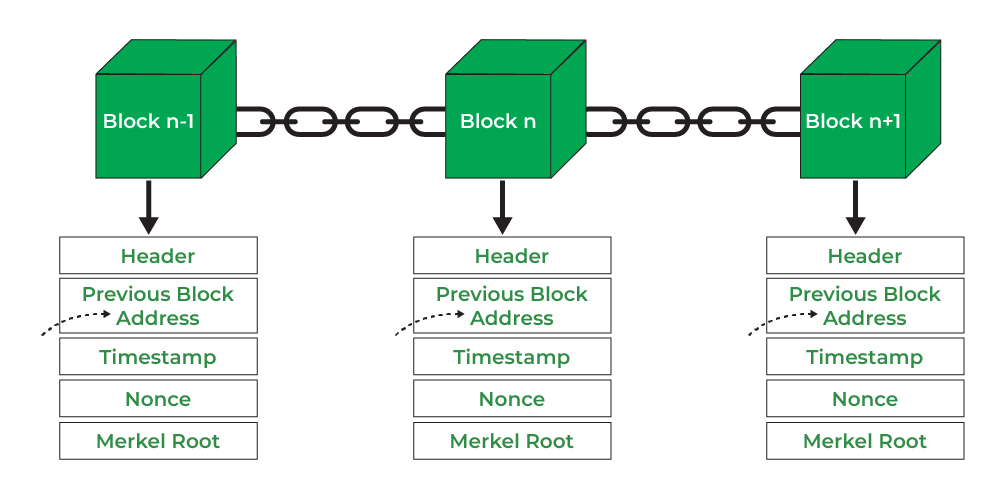
\includegraphics[scale=0.26,clip=false]{pictures/blocks.png}
  \end{center}

  If one modifies data in block $n$, then also blocks $n+1$, $n+2$, \ldots
  must be modified because otherwise the previous hash links do not match

  \medskip

  \begin{redbox}{}
    It's still possible in a few seconds for a modern computer
  \end{redbox}
  
\end{frame}

\begin{frame}\frametitle{Proof of Work}

  \begin{redbox}{}
    Cynthia Dwork and Noni Naor (1992). “Pricing via Processing, Or, Combatting Junk Mail, Advances in Cryptology”. CRYPTO’92: Lecture Notes in Computer Science No. 740. Springer: 139–147.
  \end{redbox}

  \bigskip

  \begin{tabular}{ccc}
    text of email & hashing & \\
    recipient address & $\Rightarrow$ & $\mathtt{\underbrace{0000000}43f5e6bc00d56984\ldots5974edf}$\\
    date of the email && \\
    numerical nonce &&
  \end{tabular}

  \bigskip

  The email client will accept the email only if the hash starts with at least 7 (or more) zeros

  \bigskip

  The sender needs to try and retry the hashing by changing the nonce, until it finds a good hash that will be accepted

  \bigskip

  This takes time and consumes energy: it makes spam expensive

\end{frame}

\begin{frame}\frametitle{Bitcoin = Secure chain of blocks + Proof of work}

  \begin{center}
    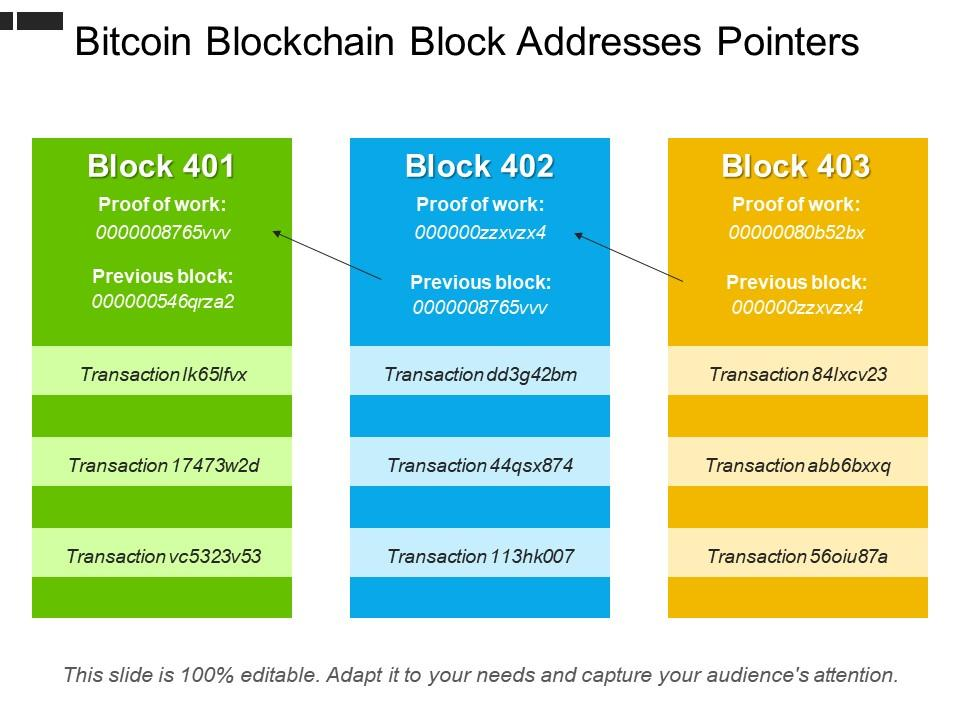
\includegraphics[scale=0.28,clip=false]{pictures/blocks-pow.jpg}
  \end{center}

  \begin{redbox}{}
    If one modifies data in block $n$, then also blocks $n+1$, $n+2$, \ldots
    must be modified because otherwise the previous hash links do not match
    and their proof of block must be recomputed: it takes centuries even on
    a very fast computer
  \end{redbox}

\end{frame}

\begin{frame}\frametitle{How to kill a dictator}

  \begin{greenbox}{Without proof of work}
    A single node dictates the history of the blockchain
    if it is faster than \emph{each} other node
  \end{greenbox}

  \pause
  \bigskip
  \bigskip

  \begin{greenbox}{With proof of work}
    A single node dictates the history of the blockchain
    if it is faster than \emph{the sum of all} other nodes
  \end{greenbox}

\end{frame}

\begin{frame}\frametitle{The magic behind the proof of work}

  \begin{greenbox}{}
    It makes expensive the production of new blocks, in time and cost (electricity)
    \begin{itemize}
    \item who produces invalid blocks sees its blocks rejected by peers and wastes resources
    \item a single node cannot drive the history, since it must fight against
      the hashing power of all other nodes together
    \item forks become unlikely, since the probability of two nodes finding a new block at the same time is small
    \end{itemize}
  \end{greenbox}

\end{frame}

\begin{frame}\frametitle{The miner computer}

  \begin{center}
    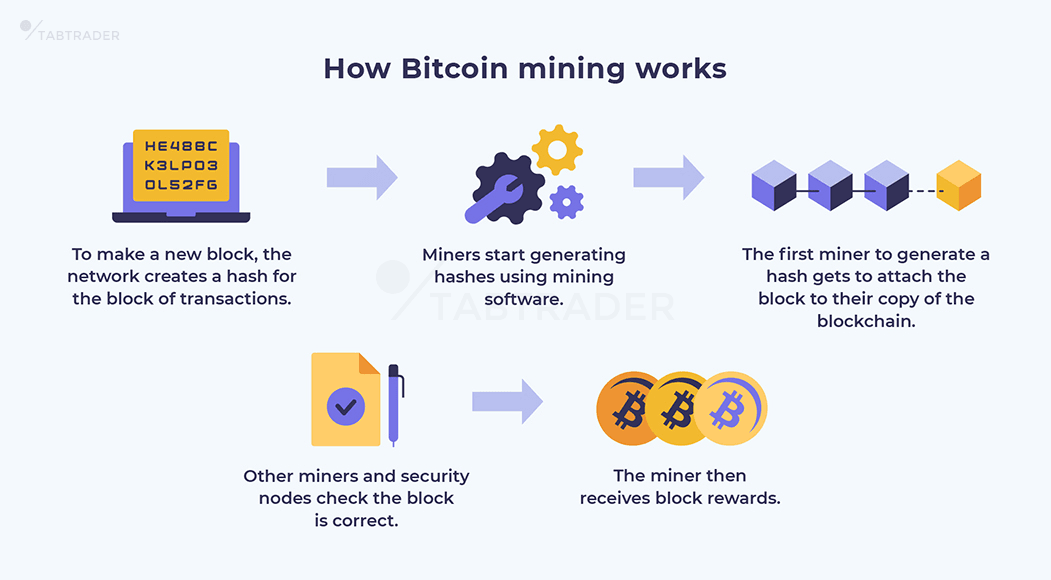
\includegraphics[scale=0.28,clip=false]{pictures/miner.png}
  \end{center}

  \begin{greenbox}{}
    Miners must be powerful computers that remain on almost continously!
  \end{greenbox}

\end{frame}

\begin{frame}\frametitle{Evolution of the miners}

  \begin{center}
    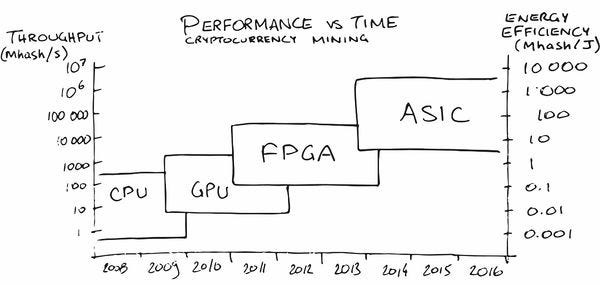
\includegraphics[scale=0.55,clip=false]{pictures/mining-hardware.jpg}
  \end{center}

\end{frame}

\begin{frame}\frametitle{Difficulty over time}

  \begin{center}
    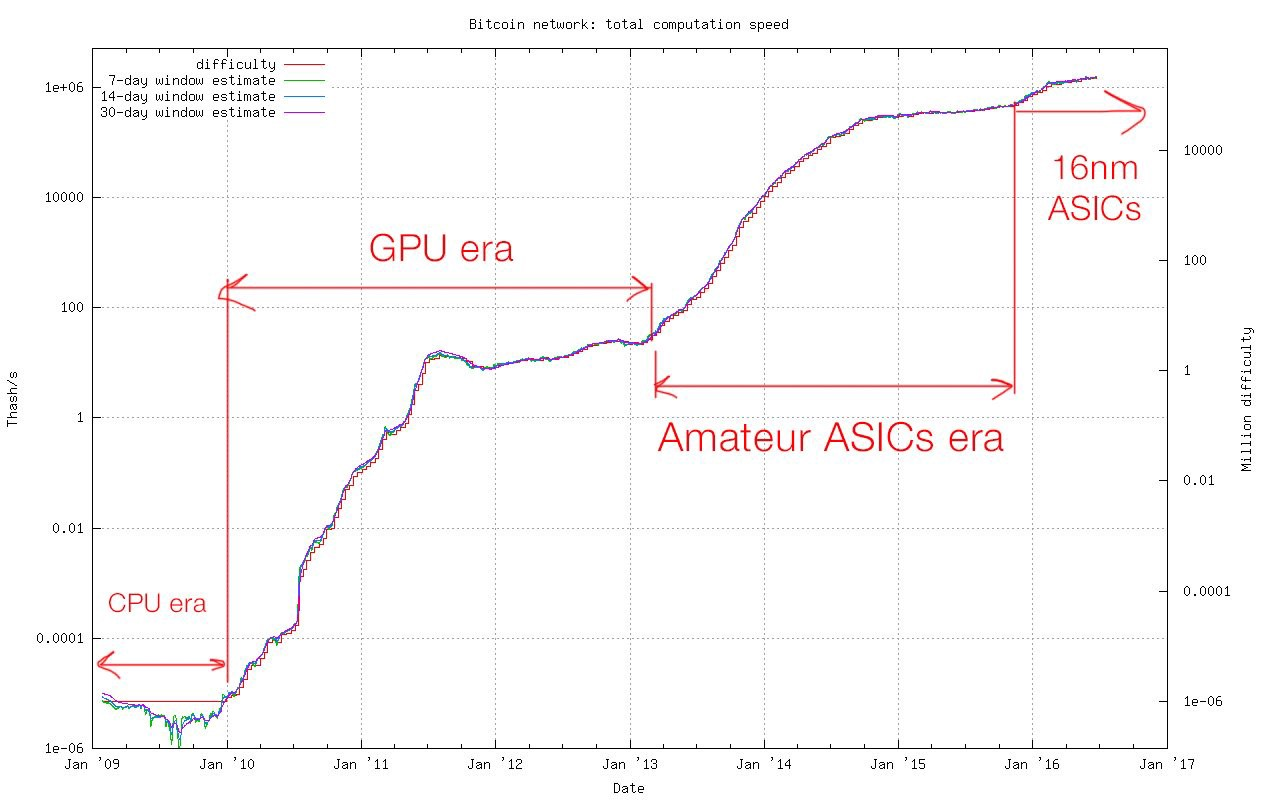
\includegraphics[width=\textwidth,clip=false]{pictures/difficulty.jpg}
  \end{center}

\end{frame}

\begin{frame}\frametitle{PoW costs electricity}

  \begin{greenbox}{2019}
    \begin{center}
      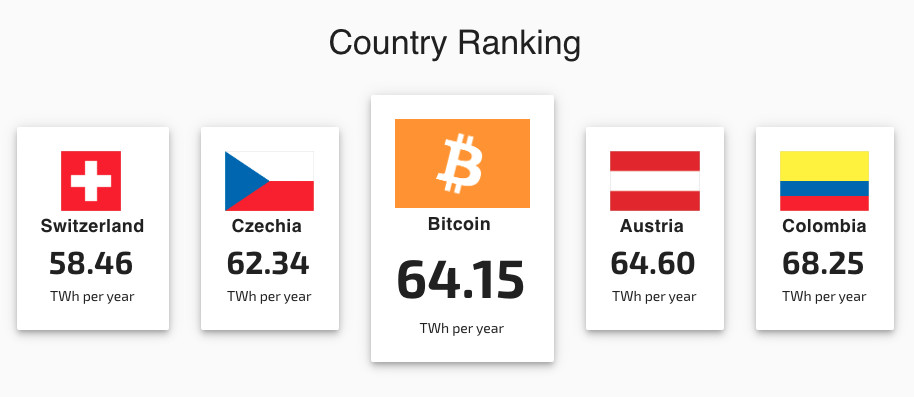
\includegraphics[scale=0.17,clip=false]{pictures/bitcoin-consumption.jpg}
      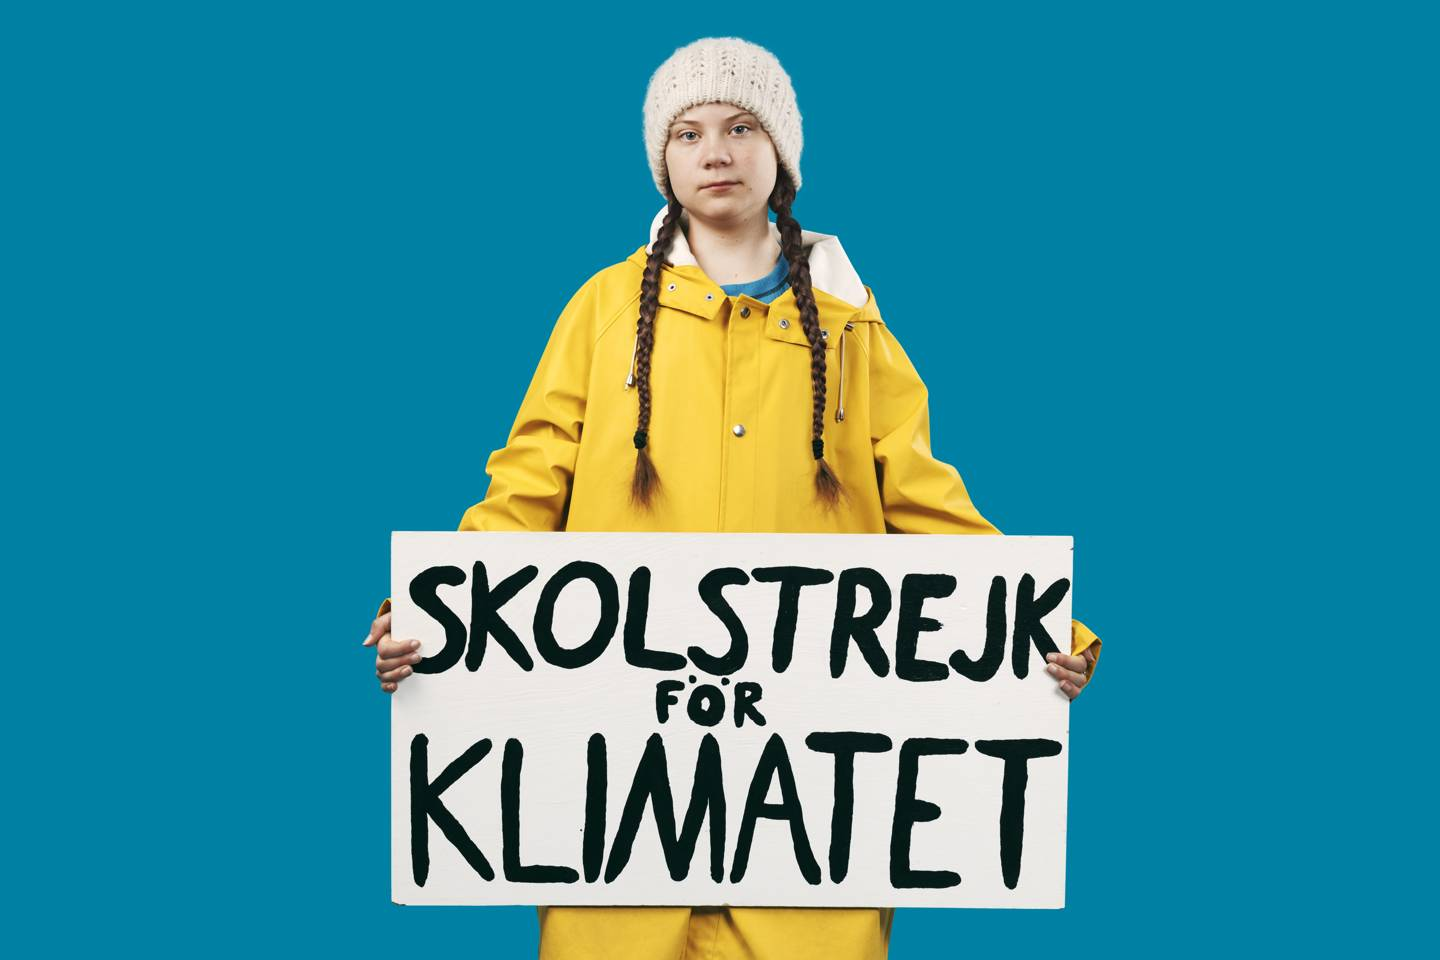
\includegraphics[scale=0.14,clip=false]{pictures/greta.jpg}
    \end{center}
  \end{greenbox}
    
\end{frame}

\begin{frame}\frametitle{Blockhains are used for cryptocurrencies}

  \begin{center}
    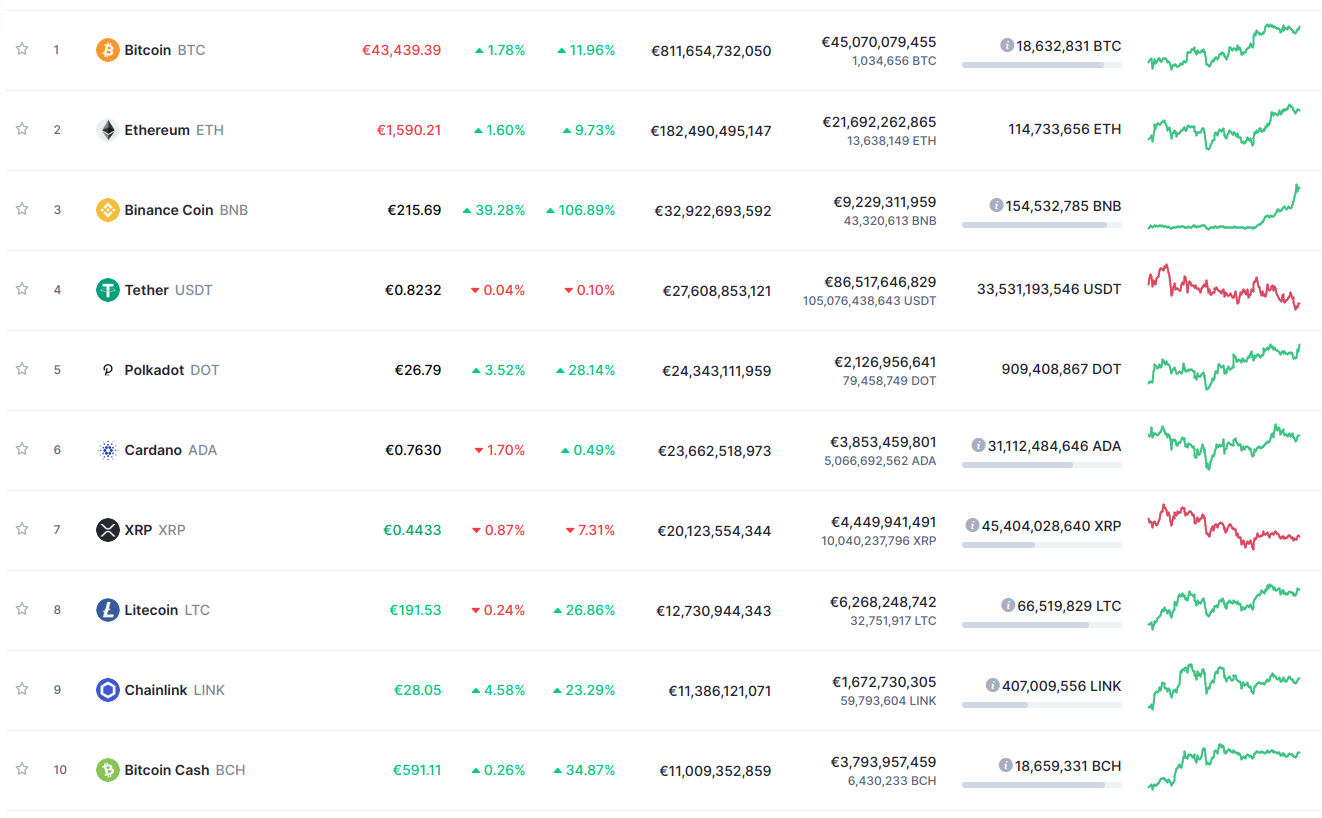
\includegraphics[scale=0.258,clip=false]{pictures/market.png}
  \end{center}

\end{frame}

\begin{frame}\frametitle{Blockhains are used for notarization}

  \begin{center}
    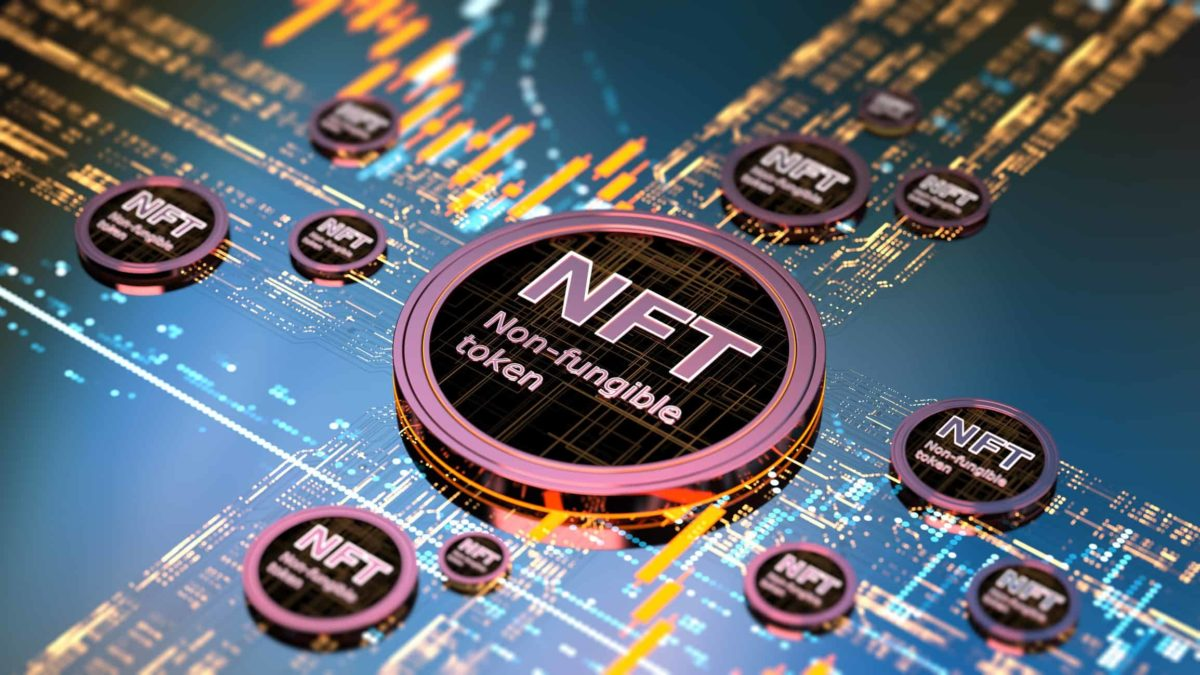
\includegraphics[scale=0.258,clip=false]{pictures/nft.jpg}
  \end{center}

\end{frame}

\begin{frame}\frametitle{Blockhains are used for ransoms}

  \begin{center}
    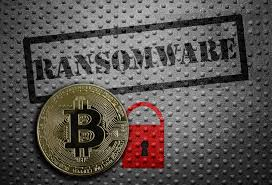
\includegraphics[scale=0.7, clip=false]{pictures/ransom.jpg}
  \end{center}

  \begin{redbox}{}
    Send one bitcoin to this account and your data will be decrypted for you
  \end{redbox}

\end{frame}

\begin{frame}\frametitle{Blockhains are used to circumvent international rules or bans}

  \begin{center}
    
\includegraphics[scale=0.5, clip=false]{pictures/send-money.jpg}
  \end{center}

\end{frame}

\begin{frame}\frametitle{Is all this worth its energy consumption and pollution?}

  \begin{center}
    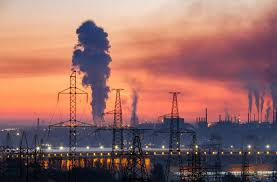
\includegraphics[scale=1, clip=false]{pictures/pollution.jpg}
  \end{center}

\end{frame}

\begin{frame}\frametitle{The best reference}

  \begin{center}
    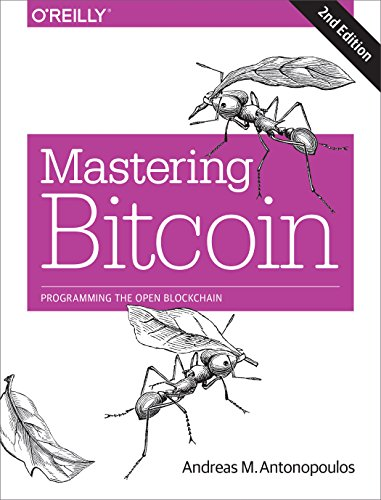
\includegraphics[scale=.35,clip=false]{pictures/mastering-bitcoin.jpg}
  \end{center}

  \begin{center}
    \url{https://github.com/bitcoinbook/bitcoinbook}
  \end{center}

\end{frame}

\begin{frame}
  \frametitle{Can blockchain work without wasting energy?}

  \begin{center}
    Who decides the next block?
  \end{center}

  \bigskip

  \begin{greenbox}{}
    \begin{itemize}
    \item proof of work [PoW] (who works harder and is lucky)
    \item proof of stake [PoS] (who commits more money)
    \item proof of space (who commits more disk space)
    \item proof of authority (who has more authority)
    \item \ldots
    \end{itemize}
  \end{greenbox}

  \bigskip

  \begin{greenbox}{PoS is a variant of Practical Byzantine Fault Tolerance (BFT)}
    Miguel Castro and Barbara Liskov.
    \emph{Practical Byzantine Fault Tolerance and Proactive Recovery}.
    ACM Trans.\ Comput.\ Syst., 20(4):398–461, November 2002
  \end{greenbox}

\end{frame}

\begin{frame}\frametitle{Tendermint (now Ignite): \url{ignite.com}}

  \begin{greenbox}{Jae Kwon. \emph{Tendermint: Consensus without Mining}, 2014.\\
    \url{https://tendermint.com/static/docs/tendermint.pdf}}
    \begin{itemize}
    \item only a dynamic set $V$ of validators decides the next block
    \item to become validator, one must block a big amount of money
    \item if a validator produces illegal blocks or misbehaves, its money will be reduced
    \end{itemize}
  \end{greenbox}

  \smallskip

  \begin{center}
    The idea is that who has money has more interest in the health of the blockchain
  \end{center}

  \smallskip

  \begin{center}
    Low energy consumption, but this is not really decentralized!
  \end{center}

\end{frame}

\begin{frame}\frametitle{Proof of stake: can we trust it?}

  \begin{greenbox}{Yes we can: Ethereum successfully moved from PoW to PoS}
    \begin{itemize}
    \item it's a special case, whose coin ETH is very valuable: validators are a serious form of investment
    \end{itemize}
  \end{greenbox}

  \bigskip
  
  \begin{redbox}{No we can't: all new blockchain projects remain borderline}
    \begin{itemize}
    \item validators initially have no interest in being validators (the coin has no value)
    \item validators are afraid of having a machine always connected and open to the internet
    \item validators find it expensive to maintain and update their machine
    \item validators lose cryptocurrency if a blackout or network failure isolate their machine
    \item please ask this question: ``How many validators your blockchain project has, where are they and who maintains such machines'' (spoiler: very few, in the same room, all maintained by one person)
    \end{itemize}
  \end{redbox}

\end{frame}

\begin{frame}
  \frametitle{Hotmoka (Fausto Spoto, 2019--2021): \url{www.hotmoka.io}}

  \begin{center}
    
\includegraphics[scale=0.2,clip=false]{pictures/hotmoka_logo.png}
  \end{center}
  
  \begin{greenbox}{}
    An open-source implementation of a network of nodes:
    \begin{itemize}
    \item nodes of a blockchain
    \item IoT devices
    \item computers in the cloud
    \end{itemize}
  \end{greenbox}

  \bigskip

  \begin{greenbox}{Requests are OO-based}
    \begin{itemize}
    \item install code in the node
    \item create an object
    \item call a method of an object
    \item methods are implemented in Takamaka (subset of Java)
    \end{itemize}
  \end{greenbox}

\end{frame}

\begin{frame}\frametitle{Hotmoka nodes \underline{can} be Tendermint applications}

  \begin{center}
    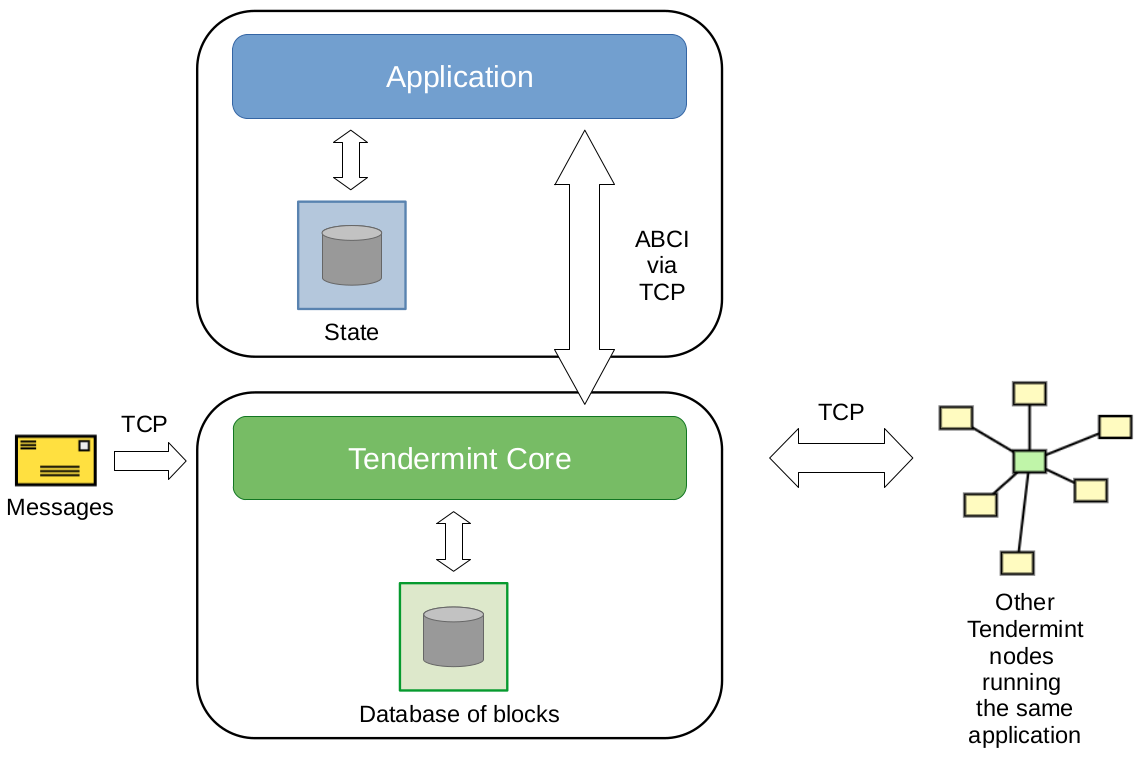
\includegraphics[width=\textwidth,clip=false]{pictures/tendermint-databases.png}
  \end{center}
    
\end{frame}

\begin{frame}{References}
  \begin{itemize}
  \item Fausto Spoto:
\emph{A Java Framework for Smart Contracts}. Financial Cryptography Workshops 2019: 122-137
  \item Fausto Spoto:
\emph{Enforcing Determinism of Java Smart Contracts}. Financial Cryptography Workshops 2020: 568-583
  \item Luca Olivieri, Fausto Spoto, Fabio Tagliaferro:
\emph{On-Chain Smart Contract Verification over Tendermint}. Financial Cryptography Workshops 2021: 333-347
  \item Marco Crosara, Luca Olivieri, Fausto Spoto, Fabio Tagliaferro:
\emph{Re-engineering ERC-20 Smart Contracts with Efficient Snapshots for the Java Virtual Machine}. BCCA 2021: 187-194, to appear in Cluster Computing
  \item Andrea Benini, Mauro Gambini, Sara Migliorini, Fausto Spoto:
\emph{Power and Pitfalls of Generic Smart Contracts}. BCCA 2021: 179-186, to appear in Cluster Computing
  \end{itemize}
\end{frame}

\begin{frame}\frametitle{Proof of space}

  \begin{itemize}
  \item proof of work is too expensive and polluting
  \item proof of stake is complex and makes it hard to have many really independent validators
  \end{itemize}

  \medskip

  \begin{greenbox}{Proof of space}
    In 2014, Burstcoin (later Signum) implemented a mining algorithm
    where miners must solve a puzzle to gain the right to mine a new block:
    \begin{itemize}
    \item the puzzle is too hard to be computed for each new block
    \item the puzzle becomes very simple if some information is precomputed and stored on disk
    \item the CPU of the miners remains largely idle: no electricity cost
    \item the more precomputation, the more disk is committed, the higher the probability of solving the puzzle and mining a new block
    \end{itemize}
  \end{greenbox}
  
\end{frame}

\begin{frame}{Mokamint (\url{www.mokamint.io})}

  Signum is monolithic, non-commented, Java 5, undocumented code

  \bigskip
  \bigskip

  \begin{greenbox}{The idea of Mokamint (Fausto Spoto 2023, work in progress)}
    \begin{itemize}
    \item Tendermint: a generic blockchain engine based on proof of stake
    \item Mokamint: a generic blockchain engine based on proof of space
      \begin{center}
        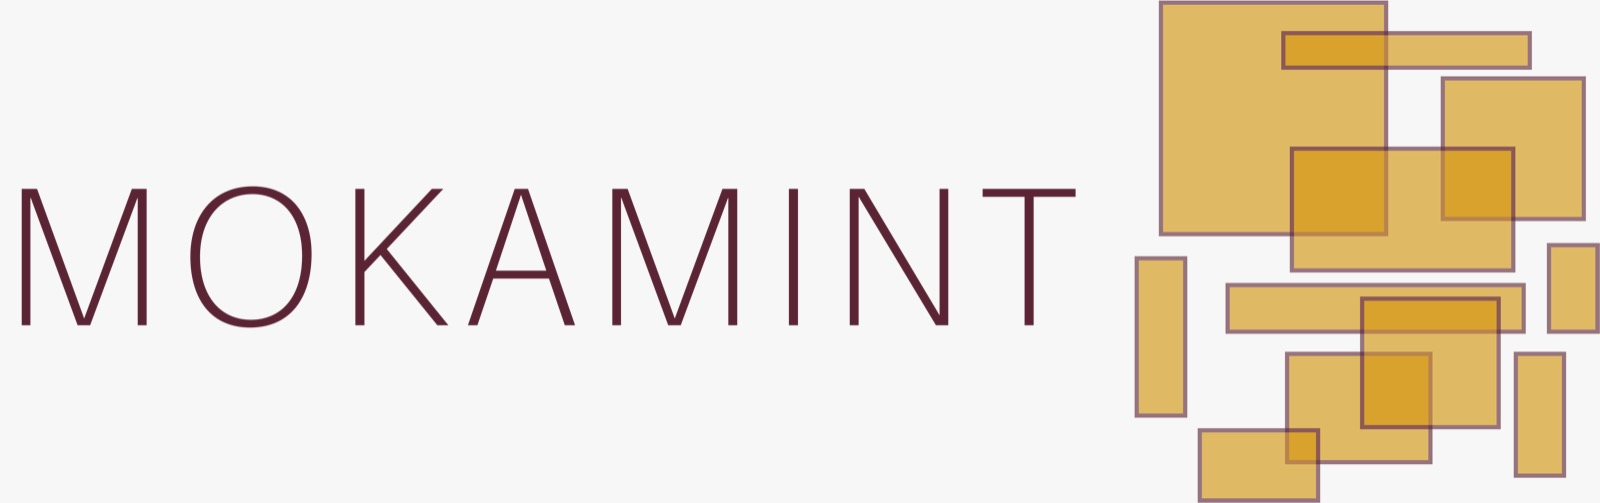
\includegraphics[scale=0.1,clip=false]{pictures/mokamint_colors.jpg}
      \end{center}
    \end{itemize}
  \end{greenbox}

  \bigskip

  Later attach Hotmoka on top of Mokamint, as an application instance

\end{frame}

\begin{frame}\frametitle{The final picture}

  \begin{center}
    \begin{tabular}{c||c|c}
      proof of work & decentralized, energy intensive & direct democracy \\\hline
      proof of stake & centralized, low energy consumption & oligarchy \\\hline
      proof of space & decentralized, low energy consumption & direct democracy
    \end{tabular}
  \end{center}
  
\end{frame}

\end{document}
